\chapter{Implementation}

%---------------------------------------------------------------
\section{Required libraries}

\hspace{15mm}To be able to write the library, I first decided to implement the dependencies: \textit{liboauth}, \textit{OpenSSL} and \textit{libcurl}.

I started by downloading liboauth. The content of the library is really simple because it consists of eight C source code and header files. I managed to compile the FreeRTOS simulator including the OAuth library: in order to do so, I first edited the simulator \textit{makefile}\footnote{A makefile is a file containing compilation instructions.} by hand.

\begin{figure}[h]
  \centering
  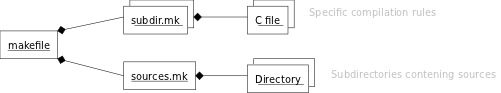
\includegraphics[scale=0.75]{images/makefile.png}
  \caption{FreeRTOS POSIX simulator, makefile architecture}
\end{figure}

As shown in the figure above, the compilation instructions are gather into a \textit{Debug} folder where rules are split into sub-files. Thus, I added a \textit{subdir.mk} listing the C source codes files of the library and I referenced the name of the sub-directory into \textit{sources.mk}.

To compile liboauth the system requires \textit{OpenSSL} and \textit{libcurl}. Therefore I added some GCC options that references these libraries into the makefile: \textit{-lssl -lcrypto -lcurl}. Nevertheless, the libraries used are those installed on my own system, not those specific to simulated FreeRTOS system, which is not suitable for an embedded environment.

The best possibility could be to port OpenSSL and libcurl to FreeRTOS in order to make liboauth totally independent of my system. These libraries are massive and require many research to be ported, moreover that was not an immediate priority under the plan, so I chose to set aside this issue until my Twitter library works.


%---------------------------------------------------------------
\section{Authentication process}

\hspace{15mm}Prior to determining the authentication process, I defined the required informations to perform it as follows:
\begin{itemize}
\item The \textit{Consumer token} allows a specific application to access data from Twitter.
\item The user login and password prove this user allows the application to access to his timeline.
\item The URL to send requests are static informations given by Twitter.
\end{itemize}
I chose to defined the \textit{Consumer token} and the user informations as parameters of the main authentication function. In this way, the developer will be able to chose which Twitter application and which Twitter account would used by the library to access data. The URL are defined as static fields into the library.

Then, the first step of the authentication is the use of the \textit{Consumer token} given by Twitter to get the \textit{Request token}. Whatever the request, the URL and sometimes the parameters are generated into a specific function according to the Twitter specifications. For this first stage:
\begin{lstlisting}
twitter_request_token_url(consumer_key, consumer_secret, &request_token_url);
twitter_request_token(request_token_url, &request_token_key, &request_token_secret, &callback);
\end{lstlisting}
Basically, the output parameters begin by the \cfunction{\&} symbol because I assign the result values to the specified variables, so I need to know its references.
For instance, the first function use the \cfunction{consumer\_key} and the \cfunction{consumer\_secret} to get the generated \cfunction{request\_token\_url}. And the second one use the \cfunction{request\_token\_url} value to return the \cfunction{request\_token\_key}, the \cfunction{request\_token\_secret} and the \cfunction{callback}.

The \textit{Verifier} step is probably the most important but also the more complex. As usual, the URL is generated by a function and then the request is sent by another one:
\begin{lstlisting}
twitter_direct_token_url(request_token_key, &direct_token_url);
twitter_verifier(direct_token_url, request_token_key, &verifier);
\end{lstlisting}
But the \cfunction{twitter\_verifier} function is divided into several steps:
\begin{itemize}
\item Send a HTTP GET request using OAuth: \cfunction{oauth\_http\_get()}.
\item Parse the HTML result of the request and get the authenticity code using \cfunction{twitter\_direct\_token\_authenticity()}.
\item Regenerate another URL and some parameters using the authenticity code, and the user account informations through \cfunction{twitter\_direct\_token\_url2()}.
\item Send a HTTP POST request using the OAuth with the new URL and the generated parameters: \cfunction{oauth\_http\_post()}.
\item Parse the HTML result of the request and get the final PIN code (or verifier) with \cfunction{twitter\_direct\_token\_pin()}.
\end{itemize}

The final step of the authentication is to obtaining the \textit{Access token}:
\begin{lstlisting}
twitter_access_token_url(consumer_key, consumer_secret, request_token_key, request_token_secret, verifier, &access_token_url);
twitter_access_token(access_token_url, &access_token_key, &access_token_secret, &access_token_user_name, &access_token_user_id);
\end{lstlisting}
These functions use the two first tokens (\textit{Consumer} and \textit{Request}) and the \textit{Verifier} to obtain the final token which could be use as a proof of user authenticity and user allowance about data accessing from his timeline.

Finally, the main function gives to the developer a C entity (typed as a structure) called \cfunction{twitterAuthEntity} and defined with the following fields:
\begin{itemize}
\item The user identifier and screen name.
\item The \textit{Consumer token} key and secret.
\item The \textit{Access token} key and secret.
\end{itemize}


%---------------------------------------------------------------
\section{Send a tweet}

\hspace{15mm}As all operations allowed by the final library, the main function require the authentication entity. Thus, this entity is one of the parameter and the fields of the structure which store the details of the authentication are used inside the function in order to perform the send operation.

The second parameter is the content of the tweet, indeed. Twitter allows to send text-based posts of up 140 characters. Other extra-details might be attached to the tweet (e.g. the geo-localisation) but this library only supports the text content.

To perform the submission, the library first generate the URL and the parameters of the HTTP POST request, and then send the tweet:
\begin{lstlisting}
twitter_tweet_url(tweet_content, consumer_key, consumer_secret, access_token_key, access_token_secret, &tweet_url, &tweet_param);
twitter_tweet(tweet_url, tweet_param, &post_result);
\end{lstlisting}

If the last function succeed, it gives the XML value of the submitted tweet. This content is parsed and returned as a \cfunction{tweet} which is typed as a structure with the following fields:
\begin{itemize}
\item The tweet identifier.
\item The creation date.
\item The user screen name.
\item The tweet text content.
\end{itemize}


%---------------------------------------------------------------
\section{Receive a tweet}

\hspace{15mm}The main function gets the entire timeline which means all tweets are received using one routine:
\begin{lstlisting}
twitter_timeline_user(consumer_key, consumer_secret, access_token_key, access_token_secret, access_token_user_name, &timeline_user);
\end{lstlisting}

The received content is in XML format and the data structure is defined as follows:

\begin{figure}[h]
  \centering
  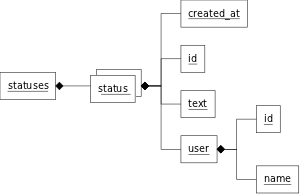
\includegraphics[scale=0.75]{images/xml.png}
  \caption{Tweets XML data structure}
\end{figure}
In the figure above, I chose to display only useful elements of the structure: those I use to fulfil \cfunction{tweet} entities.

To parse XML data I written some tool functions to count, give a value or all values from specific elements:
\begin{lstlisting}
char * xml_parser_get (const char * xml_content, const char * element_key)
int xml_parser_count (const char * xml_content, const char * element_key)
void xml_parser_getall (const char * xml_content, const char * element_key, char * element_value[])
\end{lstlisting}

Using these functions, the main one enables the developer to get an array of \cfunction{tweet}.

\clearpage